% flashcards-title: Two input-output tables
% flashcards-desc: The first table pairs one two three with four eight twelve; the second pairs one two three with four nine fourteen.
\documentclass[dvisvgm,tikz,border=8pt]{standalone}\usetikzlibrary{arrows.meta,patterns}

\definecolor{qraNavy}{HTML}{17324D}
\definecolor{qraBlue}{HTML}{2B6CB0}
\definecolor{qraGold}{HTML}{B7791F}
\definecolor{qraPale}{HTML}{EAF2F8}
\definecolor{qraGray}{HTML}{5C6773}

\tikzset{
  qra axis/.style={draw=qraNavy, line width=1.2pt},
  qra tick/.style={draw=qraNavy, line width=1pt},
  qra guide/.style={draw=qraGray, densely dashed, line width=0.8pt},
  qra counter/.style={circle, draw=qraNavy, fill=qraPale, line width=0.9pt, minimum size=7mm, inner sep=0pt},
  qra label/.style={font=\sffamily\bfseries, text=qraNavy},
  qra small label/.style={font=\sffamily, text=qraNavy},
}

\begin{document}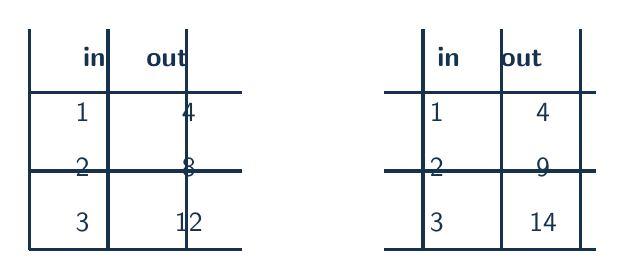
\begin{tikzpicture}[x=.9cm,y=.7cm]
\foreach \o/\vals in {0/{4,8,12},5/{4,9,14}}{\draw[qra axis](\o,0)grid(\o+3,4);\node[qra label]at(\o+1.5,3.5){in \quad out};\foreach \r/\a/\b in {1/1/4,2/2/8,3/3/12}{\node[qra small label]at(\o+.75,3.5-\r){\a};}\ifnum\o=0\foreach \r/\b in {1/4,2/8,3/12}{\node[qra small label]at(\o+2.25,3.5-\r){\b};}\else\foreach \r/\b in {1/4,2/9,3/14}{\node[qra small label]at(\o+2.25,3.5-\r){\b};}\fi}
\end{tikzpicture}\end{document}
